\section{Технологический раздел}
В данном разделе определяются средства реализации программного обеспечения, аргументируется выбор используемой СУБД и алгоритма кластеризации. Описываются данные для проведения кластеризации и приводятся сведения о модулях.

\subsection{Средства реализации программного обеспечения}
При написании программного продукта был использован язык программирования Kotlin \cite{Kotlin}.

Данный выбор обусловлен следующими факторами:
\begin{itemize}[leftmargin=1.6\parindent]
\item возможность запуска программного кода на любом устройстве, поддерживающем Java Virtual Machine;
\item большое количество актуализируемой справочной литературы, связанной как я языком программирования Java, так и Kotlin;
\item возможность интеграции программного кода в приложения для ОС Android.
\end{itemize}

При написании программного продукта использовалась среда разработки IntelliJ IDEA. Данный выбор обусловлен тем, что Kotlin является продуктом компании JetBrains, поставляющей данную среду разработки.

\subsection{Выбор СУБД}

\subsubsection{Базы данных временных рядов}
Базы данных временных рядов отличаются от статических баз данных тем, что содержат записи, в которых некоторые из атрибутов ассоциируются с временными метками. В качестве таких записей могут выступать данные мониторинга, биржевые данные о торгах или транзакции продаж. \cite{bdvrAnomalies}

\paragraph{InfluxDB}
InfluxDB - это база данных временных рядов, предназначенная для обработки высокой нагрузки записи и запросов.

Основным назначением является хранение больших объемов данных с метками времени. Например, данные мониторинга, метрики приложений и данные датчиков IoT (Internet of Things, интернет вещей).

В традиционной реляционной базе данных данные хранятся до тех пор, пока вы не решите их удалить. Учитывая сценарии использования баз данных временных рядов, можно не хранить данные слишком долго: это или слишком дорого, или данные со временем теряют актуальность. \cite{ryadi}

Системы вроде InfluxDB могут удалять данные спустя определённое время, используя концепцию, называемую политикой хранения. Также поддерживается функционал отправки непрерывных запросов к оперативным данным для выполнения определенных операций. \cite{ryadi}

\paragraph{OpenTSDB}
OpenTSDB состоит из демона временных рядов, а также набора утилит командной строки. Взаимодействие с OpenTSDB в первую очередь достигается путем запуска одного или нескольких независимых демонов.

Демон использует базу данных с открытым исходным кодом HBase или службу Google Bigtable для хранения и получения данных временных рядов. Схема данных высоко оптимизирована для быстрого объединения аналогичных временных рядов, чтобы минимизировать пространство хранения. Пользователям никогда не требуется прямой доступ к базовому хранилищу. Можно общаться с демоном через протокол telnet, HTTP API или простой встроенный графический интерфейс.

\subsubsection{Реляционные базы данных}
Реляционная база данных --- это организованный по реляционной модели набор таблиц, в которых каждая ячейка этих таблиц имеет некоторое соответствующее описание. \cite{relationki}

Использование реляционной модели предполагает возможность идентификации элементов по совокупности уникальных идентификаторов: имя столбца, первичный ключ. Для построения логической связи между строками и ячейками разных таблиц используются внешние ключи. \cite{relationki}

Среди подобных СУБД, которые основаны на реляционных базах данных выделяются: Oracle, PostgreSQL.

Каждая из указанных СУБД имеет некоторые отличительные особенности. Так, например, PostgreSQL поддерживает вставки кода, написанного на языке программирования Python, в тело процедуры. Однако выделить среди данных особенностей важных для данной работы не представляется возможным.

\subsubsection*{Вывод}
Базы данных временных рядов являются наиболее подходящими для решаемой задачи, так как они нацелены на хранение, извлечение и анализ большого количества статистических данных, в которых имеются временные метки.

Для организации хранения данных будет использоваться СУБД InfluxDB, так как она является одной из самых популярных, среди известных баз данных временных рядов, а также по той причине, что поддержка данной СУБД все еще не прекращена на сегодняшний день.

\subsection{Выбор алгоритма кластеризации}
В качестве используемого алгоритма кластеризации был выбран метод c-средних в силу того, что число кластеров заранее известно, а также задача рассматривает установку соответствия некоторого объекта (например, значения скорости печати) набора вещественных значений, показывающих степень отношения объекта к кластерам.

\subsection{Данные для кластеризации}
В качестве данных для кластеризации используются действия оператора автоматизированного рабочего места, производимые с использованием клавиатуры и мыши. Данные действия логируются с использованием программного обеспечения, а затем направляются в базу данных для возможности миграции определенной модели поведения на другое автоматизированное место.

Действия пользователя, участвующие в построении модели, соотносятся с временем реакции, которое фиксируется каждые 20 минут, причем по времени реакции определяется, в каком состоянии в текущий момент времени находится организм оператора.

\subsection{Сведения о модулях}
Программное обеспечение состоит из модулей логирования действий \newline оператора, обработки и анализа данных. Также определен модуль, который позволяет развернуть сервер для хранения данных пользователей с использованием базы данных InfluxDB.

\subsubsection{Модуль логирования действий оператора}
Данный модуль предназначен для записи информации о действиях оператора.

Библиотеки, используемые в модуле:

\begin{itemize}[leftmargin=1.6\parindent]
\item Java Swing \cite{swing} --- библиотека легковесных компонентов для реализации оконного интерфейса приложения;
\item JNativeHook \cite{jnativehook} --- библиотека, предоставляющая средства перехвата прерываний, поступающих от клавиатуры и мыши.
\end{itemize}

Исходный код модуля предоставлен в приложении 1.

Модуль состоит из четырех пакетов.

\paragraph{Пакет window \newline}
Данный пакет включает в себя абстрактный класс Window, предоставляющий родительский класс с определенными свойствами для всех окон реализуемого программного обеспечения. Реализация приведена в листинге \ref{lst:windowkt} (приложение А, с. \pageref{chp:application-a}).

\paragraph{Пакет bigBrother \newline}
Данный пакет включает в себя класс BigBrotherWindow, который является реализацией класса Window и определяет функционал главного экрана приложения. Реализация приведена в листинге \ref{lst:bigbrotherwindowkt} (приложение А, с. \pageref{chp:application-a}).

\paragraph{Пакет loggers \newline}
Данный пакет включает в себя пакеты реализаций логирующих классов: Key\-Logger (нажатия на клавиши клавиатуры), MouseLogger (нажатия на клавиши мыши и движения данного устройства), ReactionLogger (результаты пройденных тестов на реакцию). Реализация классов приведена в листингах \ref{lst:loggerkt} -- \ref{lst:reactionloggerkt} (приложение А, с. \pageref{chp:application-a}).


Также в данном пакете предоставлена реализация класса ReactionTest\-Window, предоставляющая интерфейс и логику определения реакции пользователя по нажатию на кнопку, появляющуюся в случайные моменты времени (от 2 до 10 секунд). Код приведен в листинге \ref{lst:reactiontestwindowkt} (приложение А, с. \pageref{chp:application-a}).

Каждый логирующий класс локально создает текстовый файл, в который записывает в определенном формате собранные данные. Для исключения попыток изменения файла конкурирующими потоками в каждом из них представлена реализация очереди записи, которая переносится в файл при достижения размера в сотню записей, либо по завершению работы приложения.

\paragraph{Пакет random \newline}
Данный пакет включает в себя класс, реализованный по паттерну ``Одиночка'', предоставляющий доступ к классу Random, инициализированного отложено. Данный класс используется преимущественно для получения данных о реакции пользователя. Реализация класса представлена в листинге \ref{lst:bbrandomkt} (приложение А, с. \pageref{chp:application-a}).

Также в модуле определен файл main.kt, который является точкой входа в приложения. Код файла представлен в листинге \ref{lst:mainkt} (приложение А, с. \pageref{chp:application-a}).

На рисунке \ref{fig:loggingUml} предоставлена диаграмма классов модуля.
\begin{figure}[H]
	\centering
	\includegraphics[width=\textwidth]{img/logger.pdf}
	\caption{Диаграмма классов модуля логирования.}
	\label{fig:loggingUml}
\end{figure}

%\begin{itemize}[leftmargin=1.6\parindent]
%\item bigBrother:
%	\begin{itemize}[leftmargin=1.6\parindent]
%	\item BigBrotherWindow;
%	\end{itemize}
%\item loggers:
%	\begin{itemize}[leftmargin=1.6\parindent]
%	\item keyLogger:
%		\begin{itemize}[leftmargin=1.6\parindent]
%		\item KeyLogger;
%		\end{itemize}
%	\item mouseLogger:
%		\begin{itemize}[leftmargin=1.6\parindent]
%		\item MouseLogger;
%		\end{itemize}
%	\item reactionTest:
%		\begin{itemize}[leftmargin=1.6\parindent]
%		\item ReactionLogger;
%		\item ReactionLoggerTestWindow;
%		\end{itemize}
%	\item Logger;
%	\end{itemize}
%\item random:
%	\begin{itemize}[leftmargin=1.6\parindent]
%	\item BBRandom;
%	\end{itemize}
%\item window:
%	\begin{itemize}[leftmargin=1.6\parindent]
%	\item Window;
%	\end{itemize}
%\item main.
%\end{itemize}

\paragraph{Пакет window \newline}
Данный пакет включает в себя абстрактный класс Window, предоставляющий родительский класс с определенными свойствами для всех окон реализуемого программного обеспечения. Реализация приведена в листинге \ref{lst:windowkt} (приложение А, с. \pageref{chp:application-a}).
\subsubsection{Модуль обработки данных}
Модуль синтаксического анализа данных предоставляет функции приведения записанных текстовых данных к определенным классам моделей данных.

Модуль обработки данных включает в себя два пакета: синтаксического анализа данных и приведения данных.

\paragraph{Пакет bbParser.models \newline}
Данный пакет включает в себя модели данных.

В листинге \ref{lst:modelkt} (приложение А, с. \pageref{chp:application-a}) представлена реализация абстрактного класса модели, в листингах \ref{lst:keymodelkt} -- \ref{lst:reactionmodelkt} (приложение А, с. \pageref{chp:application-a}) представлены примеры конкретных моделей.

\paragraph{Пакет bbParser.parsers \newline}
Данный пакет включает в себя синтаксические анализаторы для получаемых текстовых данных.

В листинге \ref{lst:bbparserkt} (приложение А, с. \pageref{chp:application-a}) представлена реализация абстрактного класса синтаксического анализатора. В листинге \ref{lst:keysbbparserkt} (приложение А, с. \pageref{chp:application-a}) представлен пример конкретного анализатора.

\paragraph{Пакет bbConverter \newline}
Данный пакет отвечает за получение требуемых характеристик от полученных данных, например, скорости печати.

В листинге \ref{lst:converterkt} (приложение А, с. \pageref{chp:application-a}) представлена реализация абстрактного класса. В листинге \ref{lst:keysconverterkt} (приложение А, с. \pageref{chp:application-a}) и \ref{lst:clicksconverterkt} (приложение А, с. \pageref{chp:application-a}) --- примеры преобразователей.

На рисунке \ref{fig:processingUml} предоставлена диаграмма классов модуля.
\begin{figure}[H]
	\centering
	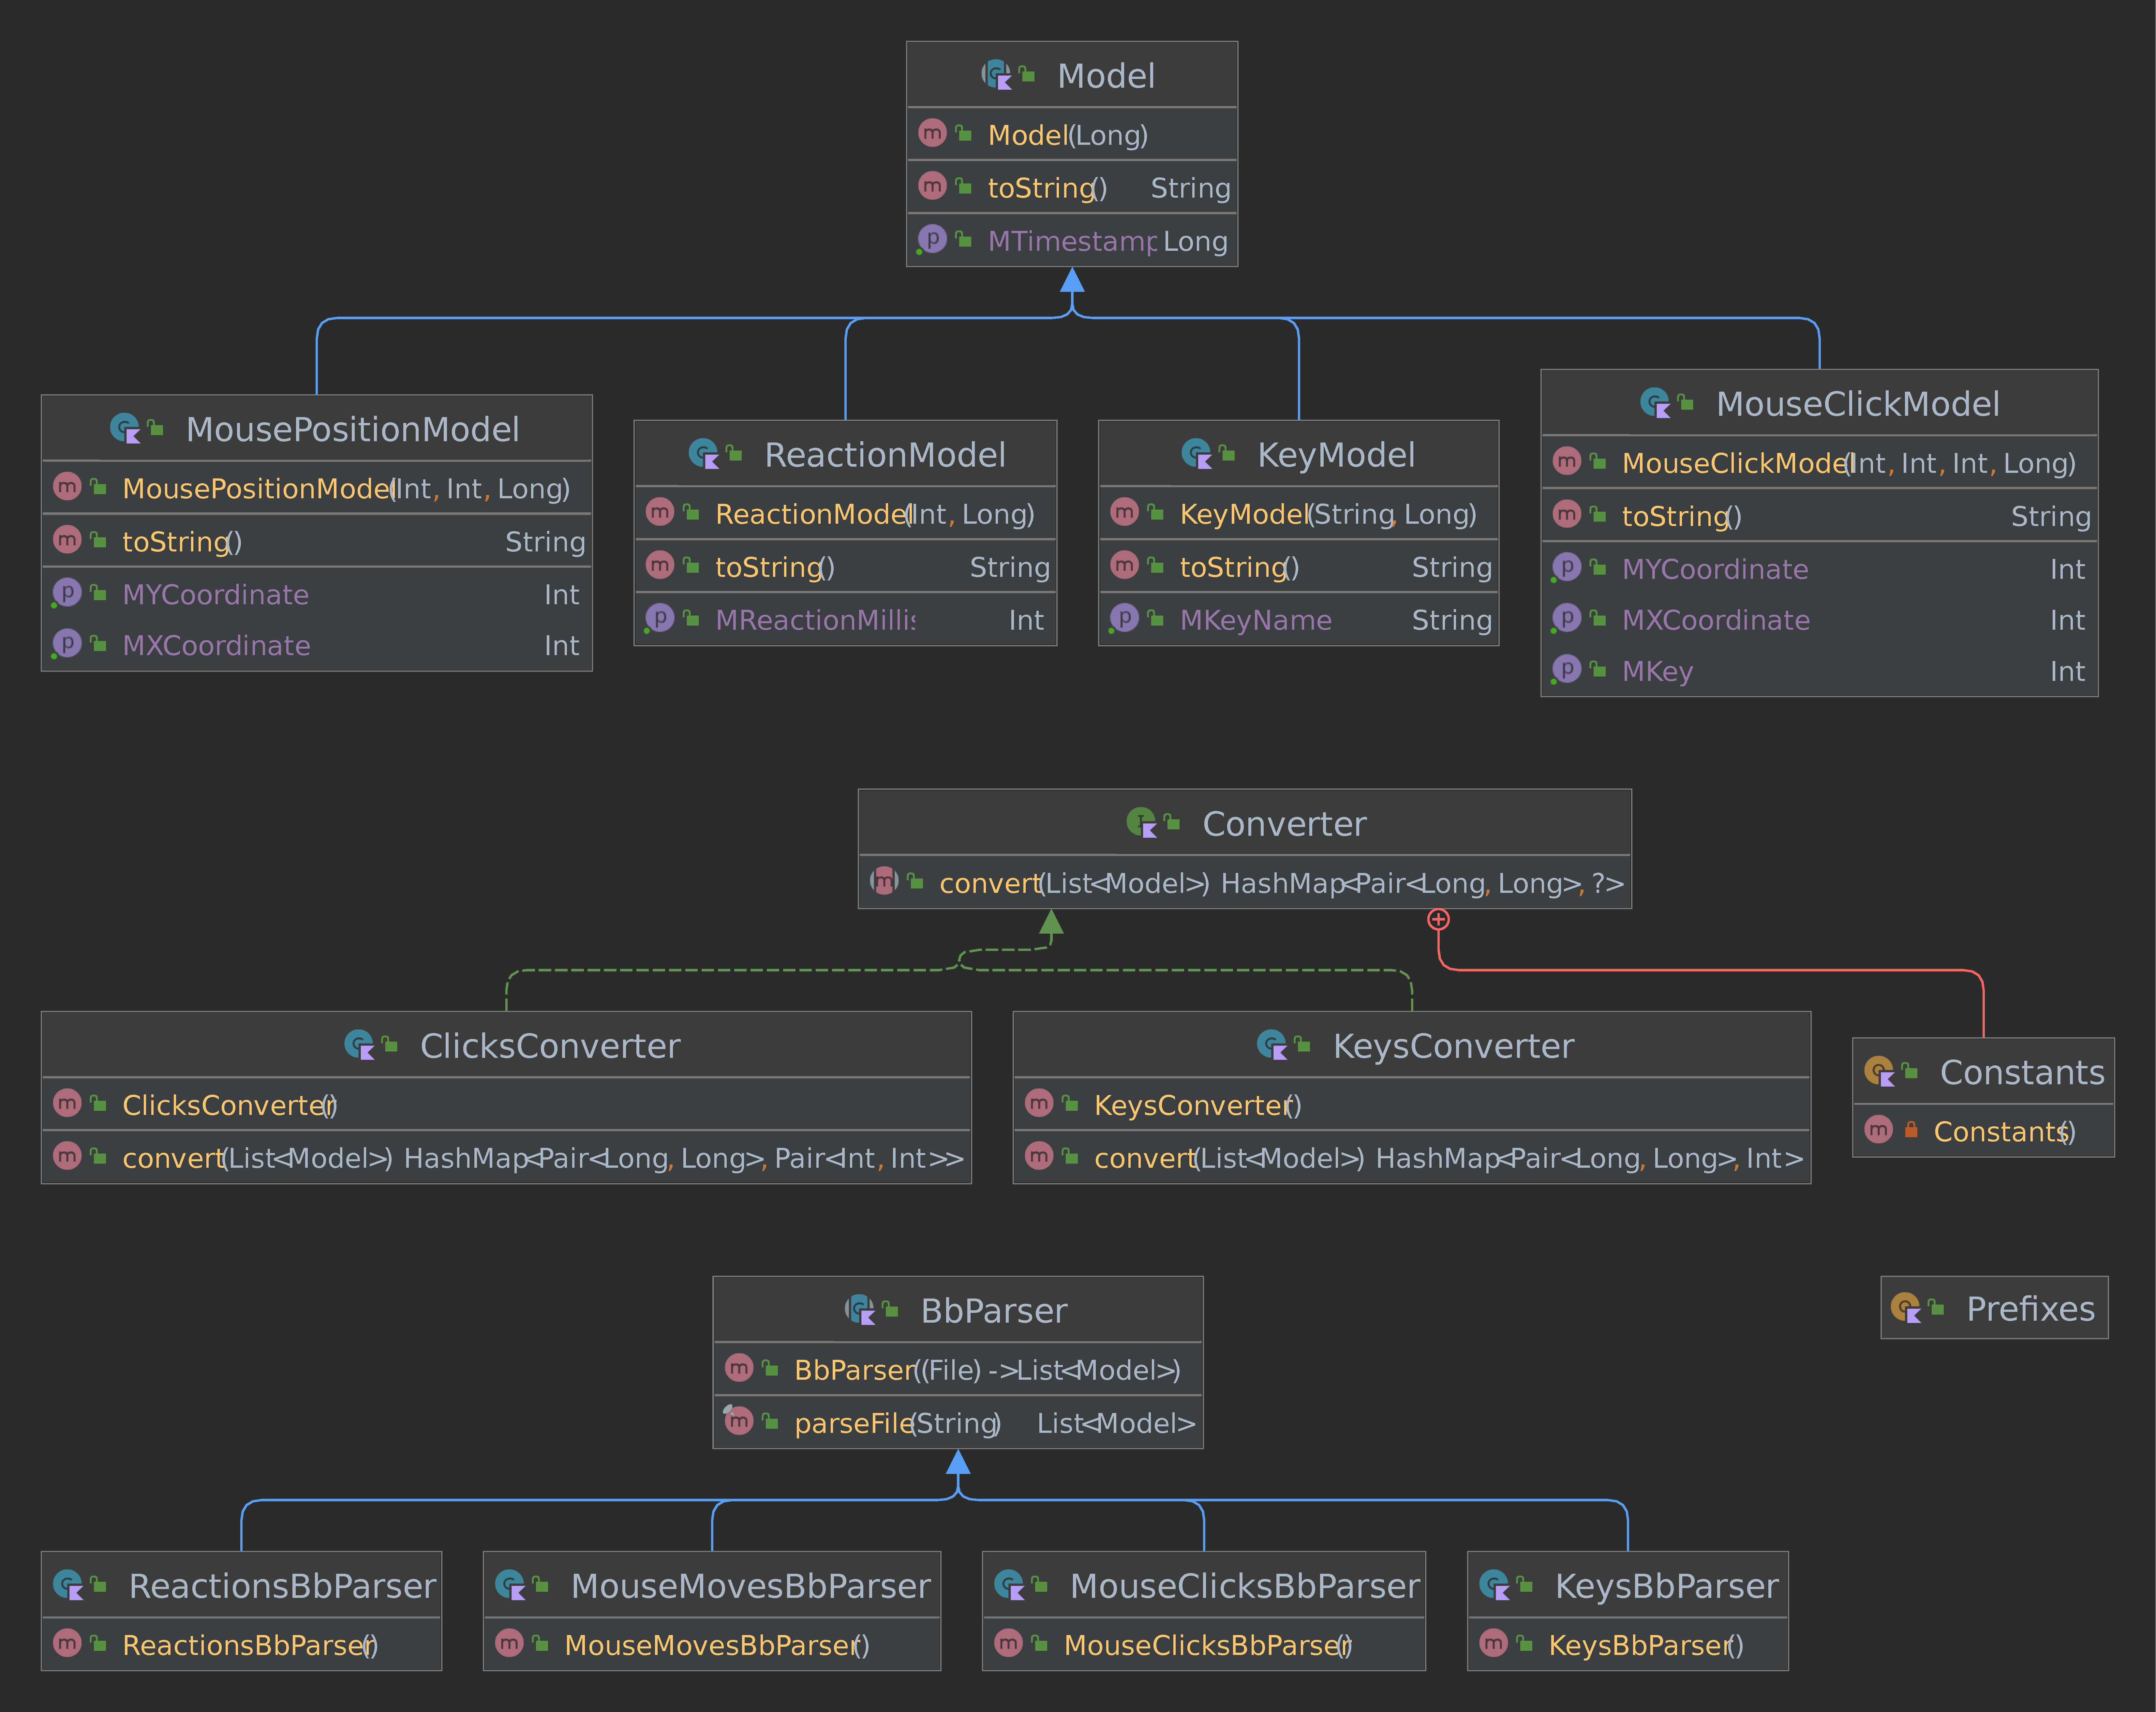
\includegraphics[width=\textwidth, angle = 90]{img/processing.pdf}
	\caption{Диаграмма классов модуля обработки данных.}
	\label{fig:processingUml}
\end{figure}

\subsubsection{Модуль анализа данных}
Данный модуль предназначен для анализа поступающих от оператора \newline данных: кластеризации данных для модели и непосредственно текущей оценки усталости оператора.

Единственной библиотекой, используемой в модуле является \foreignlanguage{english}{The Commons Mathematics Library} \cite{apachemath3}, из которой была взята реализация алгоритма кластеризации ``с-средних''.

\paragraph{Пакет analyze.clusterization \newline}

Данный пакет включает в себя утилиты для кластеризации данных, в нем представлен абстрактный класс Clusterer и его реализация BbClusterer, предоставляющий возможность определения нечетких кластеров по переданным \newline данным. Также в пакете приведен класс точки для кластеризации, используемая библиотекой The Commons Mathematics Library. Реализация приведена в листингах \ref{lst:clustererkt} --- \ref{lst:bbclustererkt} (приложение А, с. \pageref{chp:application-a}).

\paragraph{Пакет analyze.analyzers}

Данный пакет включает в себя анализаторы, позволяющие построить модель и оценивать состояние оператора с использованием различных способов предоставления данных. В листингах \ref{lst:analyzerkt} (приложение А, с. \pageref{chp:application-a}) и \ref{lst:bbanalyzerkt} (приложение А, с. \pageref{chp:application-a}) предоставлены абстрактный класс анализатора и его реализация для работы с файлами.

\paragraph{Пакет analyze.fileAnalyzer}
Данный пакет предоставляет реализацию класса, позволяющего полноценно создать модель по заданным файлам и определить состояния оператора. Реализация представлена в листинге \ref{lst:bbfileanalyzerkt} (приложение А, с. \pageref{chp:application-a}).

На рисунке \ref{fig:analyzerUml} предоставлена диаграмма классов модуля.

\begin{figure}[H]
	\centering
	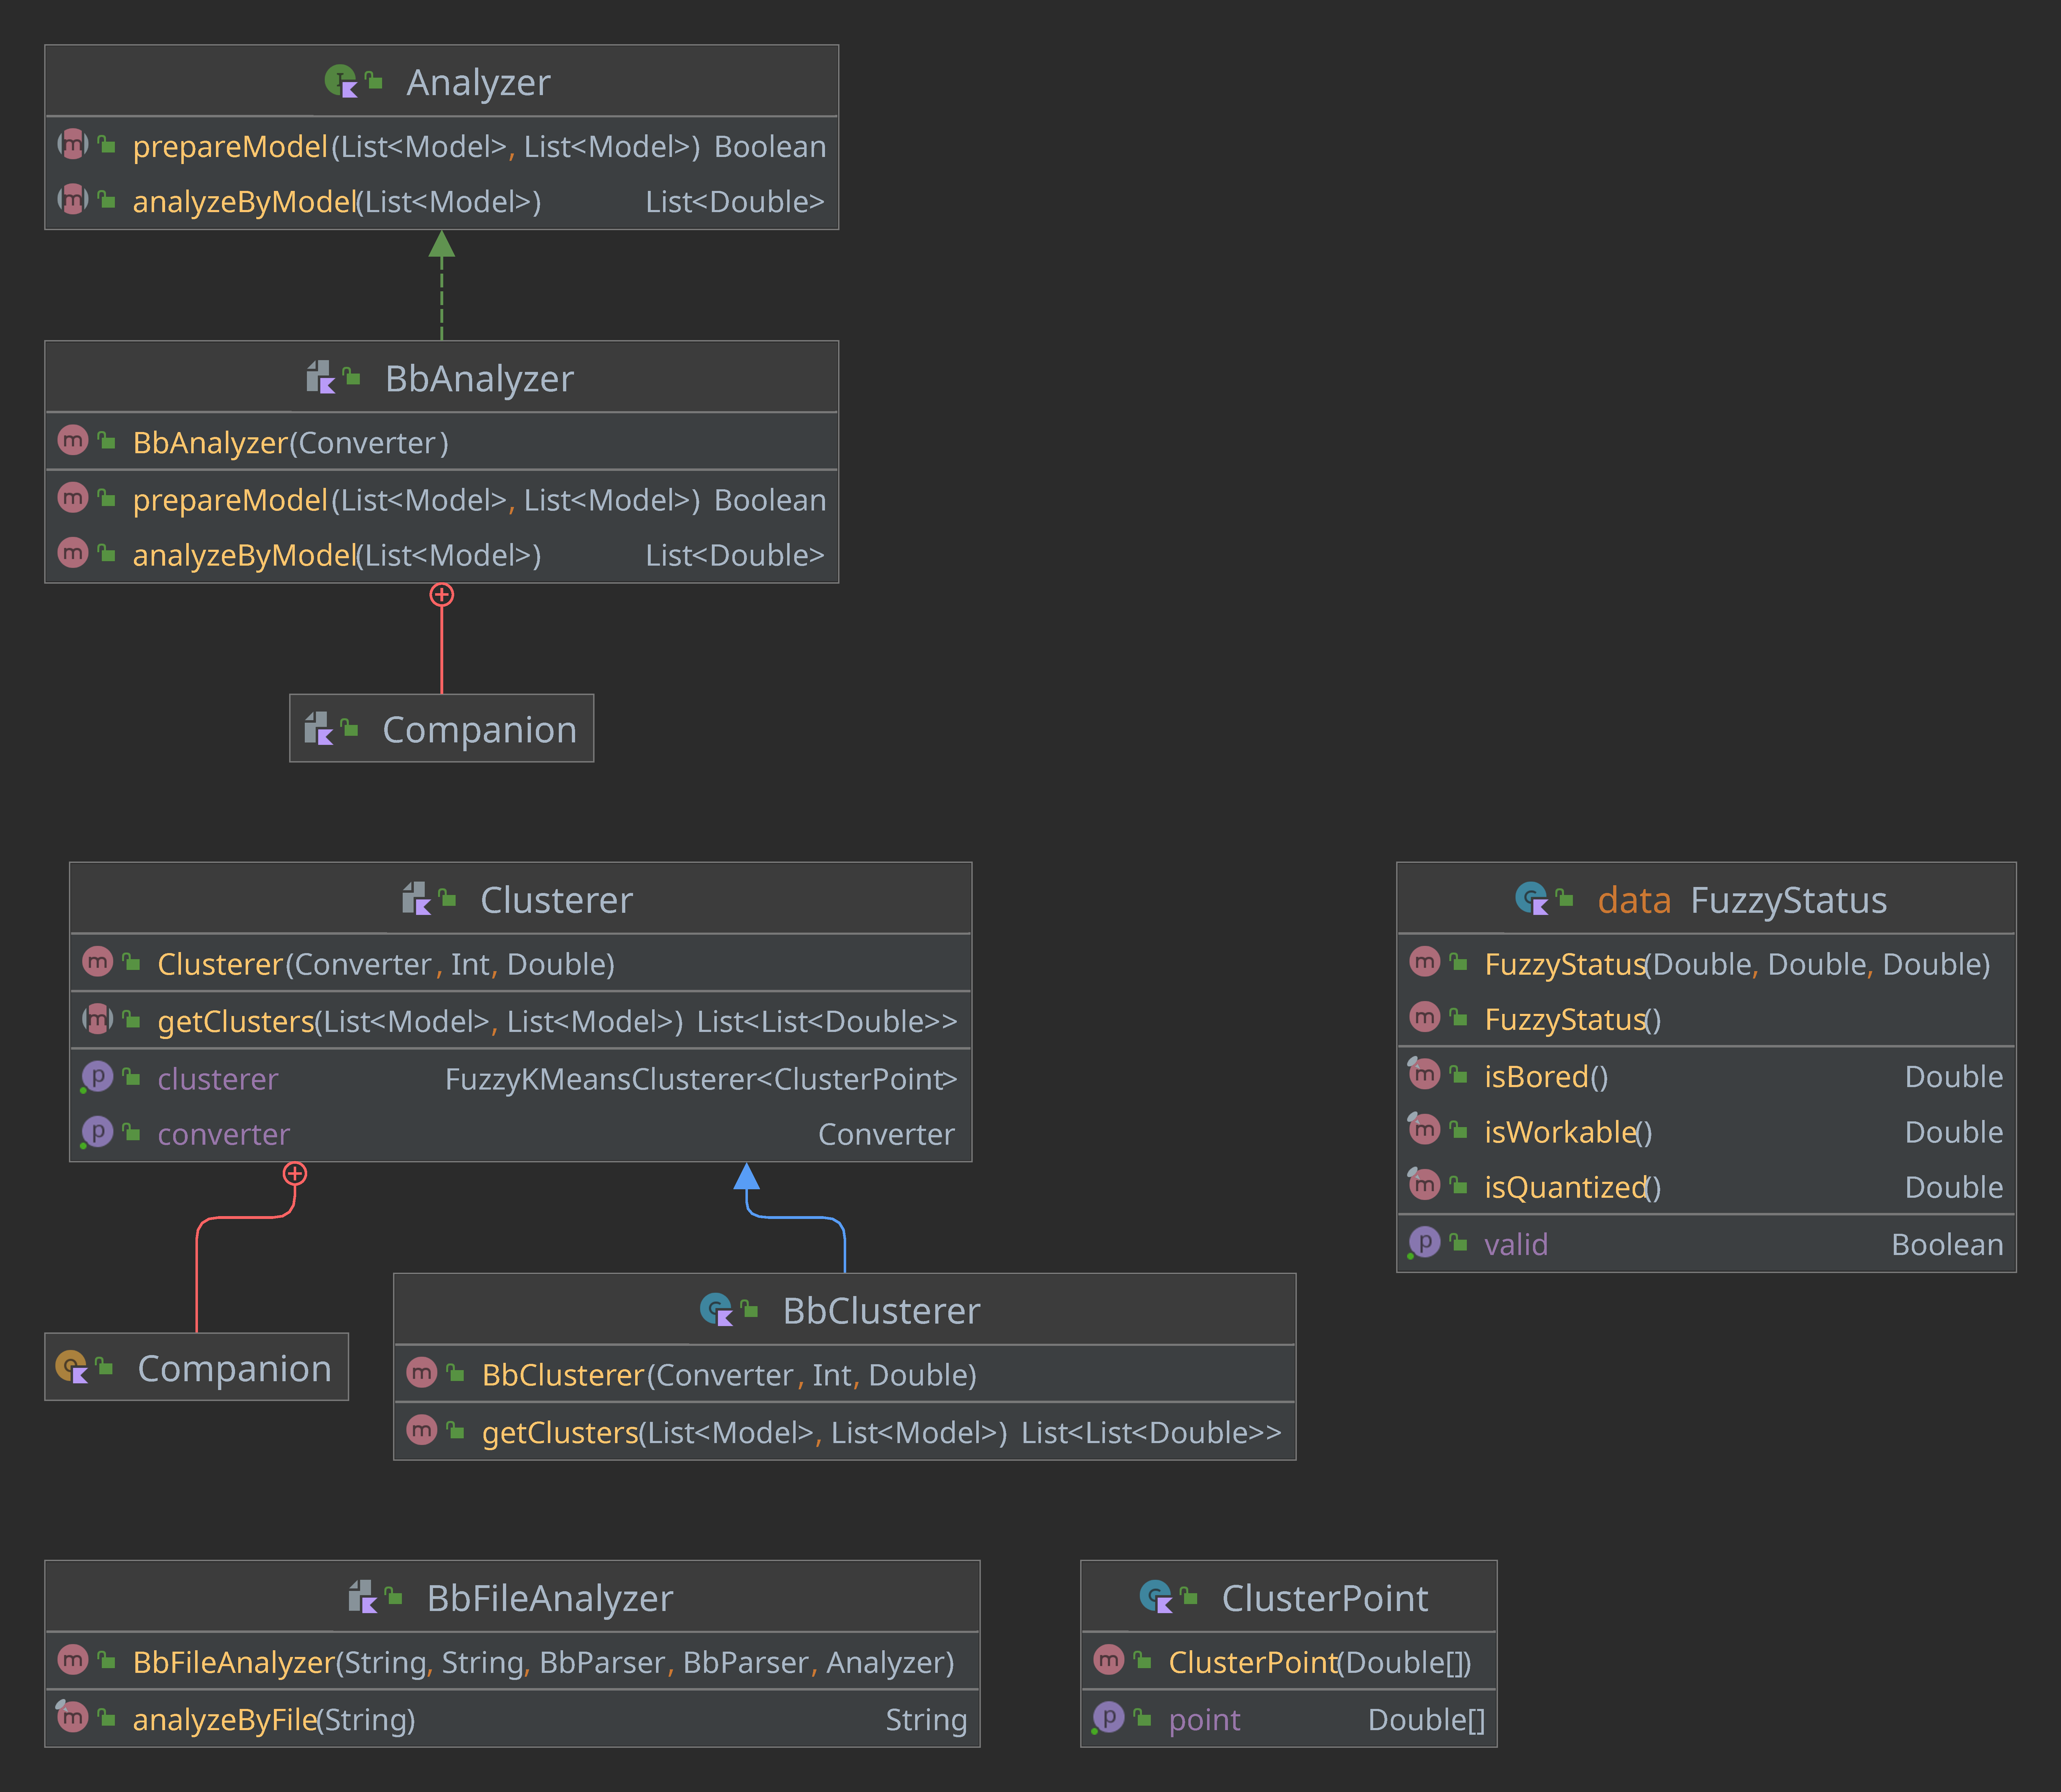
\includegraphics[width=\textwidth]{img/analyze.pdf}
	\caption{Диаграмма классов модуля анализа данных.}
	\label{fig:analyzerUml}
\end{figure}

\subsubsection{Модуль серверного приложения}
В данном модуле описана серверная составляющая хранилища данных, полученных от оператора. Главным назначением является хранение данных, позволяющих построить модель для пользователя, в случае их утраты в локальном хранилище.

Данный модуль логически разделен на следующие части:

\begin{itemize}[leftmargin=1.6\parindent]
\item пакет доступа к данным;
\item пакет бизнес-логики;
\item пакет реализации протокола;
\item пакет клиента;
\item пакет сервера.
\end{itemize}

\paragraph{Пакет доступа к данным \newline}
Данный пакет включает в себя реализацию двух классов: CharRepositoryImpl, основанного на шаблоне проектирования ``Репозиторий'', и InfluxDAO, основаного на шаблоне проектирования ``Объект доступа к данным''. Объъект доступа к данным позволяет сделать репозиторий независимым от реализации исполенния запросов к базе данных. Данный объект использует InfluxDB-client-kotlin \cite{influxClientKotlin} для запросов на внесение и чтение записей, однако отдельный функционал реализован через отправку HTTP-запросов напрямую к серверу InfluxDB с использованием OkHttp3 \cite{OkHttp}.

\paragraph{Пакет бизнес-логики \newline}
Данный пакет включает в себя множество сущностей, фигурирующих между слоями клиент-серверной архитектуры.

\paragraph{Пакет реализации протокола \newline}
Данный пакет включает в себя класс YDVP, который может представлять собой YDVP-запрос или YDVP-ответ, единственным отличием для них будет интерпретация абстрактного класса YdvvpStartingLine, от которого наследуются классы YdvpStartingLineRequest и YdvpStartingLineRespone. Данный пакет также содержит класс YdvpParser, который предоставляет функционал парсинга приходящих YDVP-запросов.

YDVP --- собственный протокол приложения, основанный на версии \newline HTTP 1.1.

\paragraph{Пакет клиента \newline}
Данный пакет включает в себя класс InfluxServiceClient, который позволяет подключиться к удалунному серверу, направлять ему YDVP-запросы и получать ответы.

\paragraph{Пакет сервера \newline}

Данный пакет включает в себя все необходимое для запуска сервера на заданном порту устройства.

В листинге \ref{lst:influxserviceserver} () представлено описание класса сервера приложения. Данный класс инициализирует классы для инъекции зависимостей в модули, используемые сервисами и котроллерами, а также передает приходящих клиентов обработчик в отдельном потоке, таким образом достигается возможность одновременной обработки запросов от нескольких клиентов.

В листинге \ref{lst:influxserviceclienthandler} (приложение Б, с. \pageref{chp:application-b}) представлено описание класса обработчика запроса клиента. Данный класс включает в себя необходимый для навигации по ресурсам контроллер, а также типовые объекты YDVP-ответов и методы обработки запроса клиента.

В листингах \ref{lst:serverExample} и \ref{lst:clientExample} (приложение Б, с. \pageref{chp:application-b}) представлен пример реализации взаимодействия пользователя с сервером.

На рисунках \ref{fig:dostup} --- \ref{fig:server} представлены диаграммы классов компонентов модуля.

\begin{figure}[H]
	\centering
	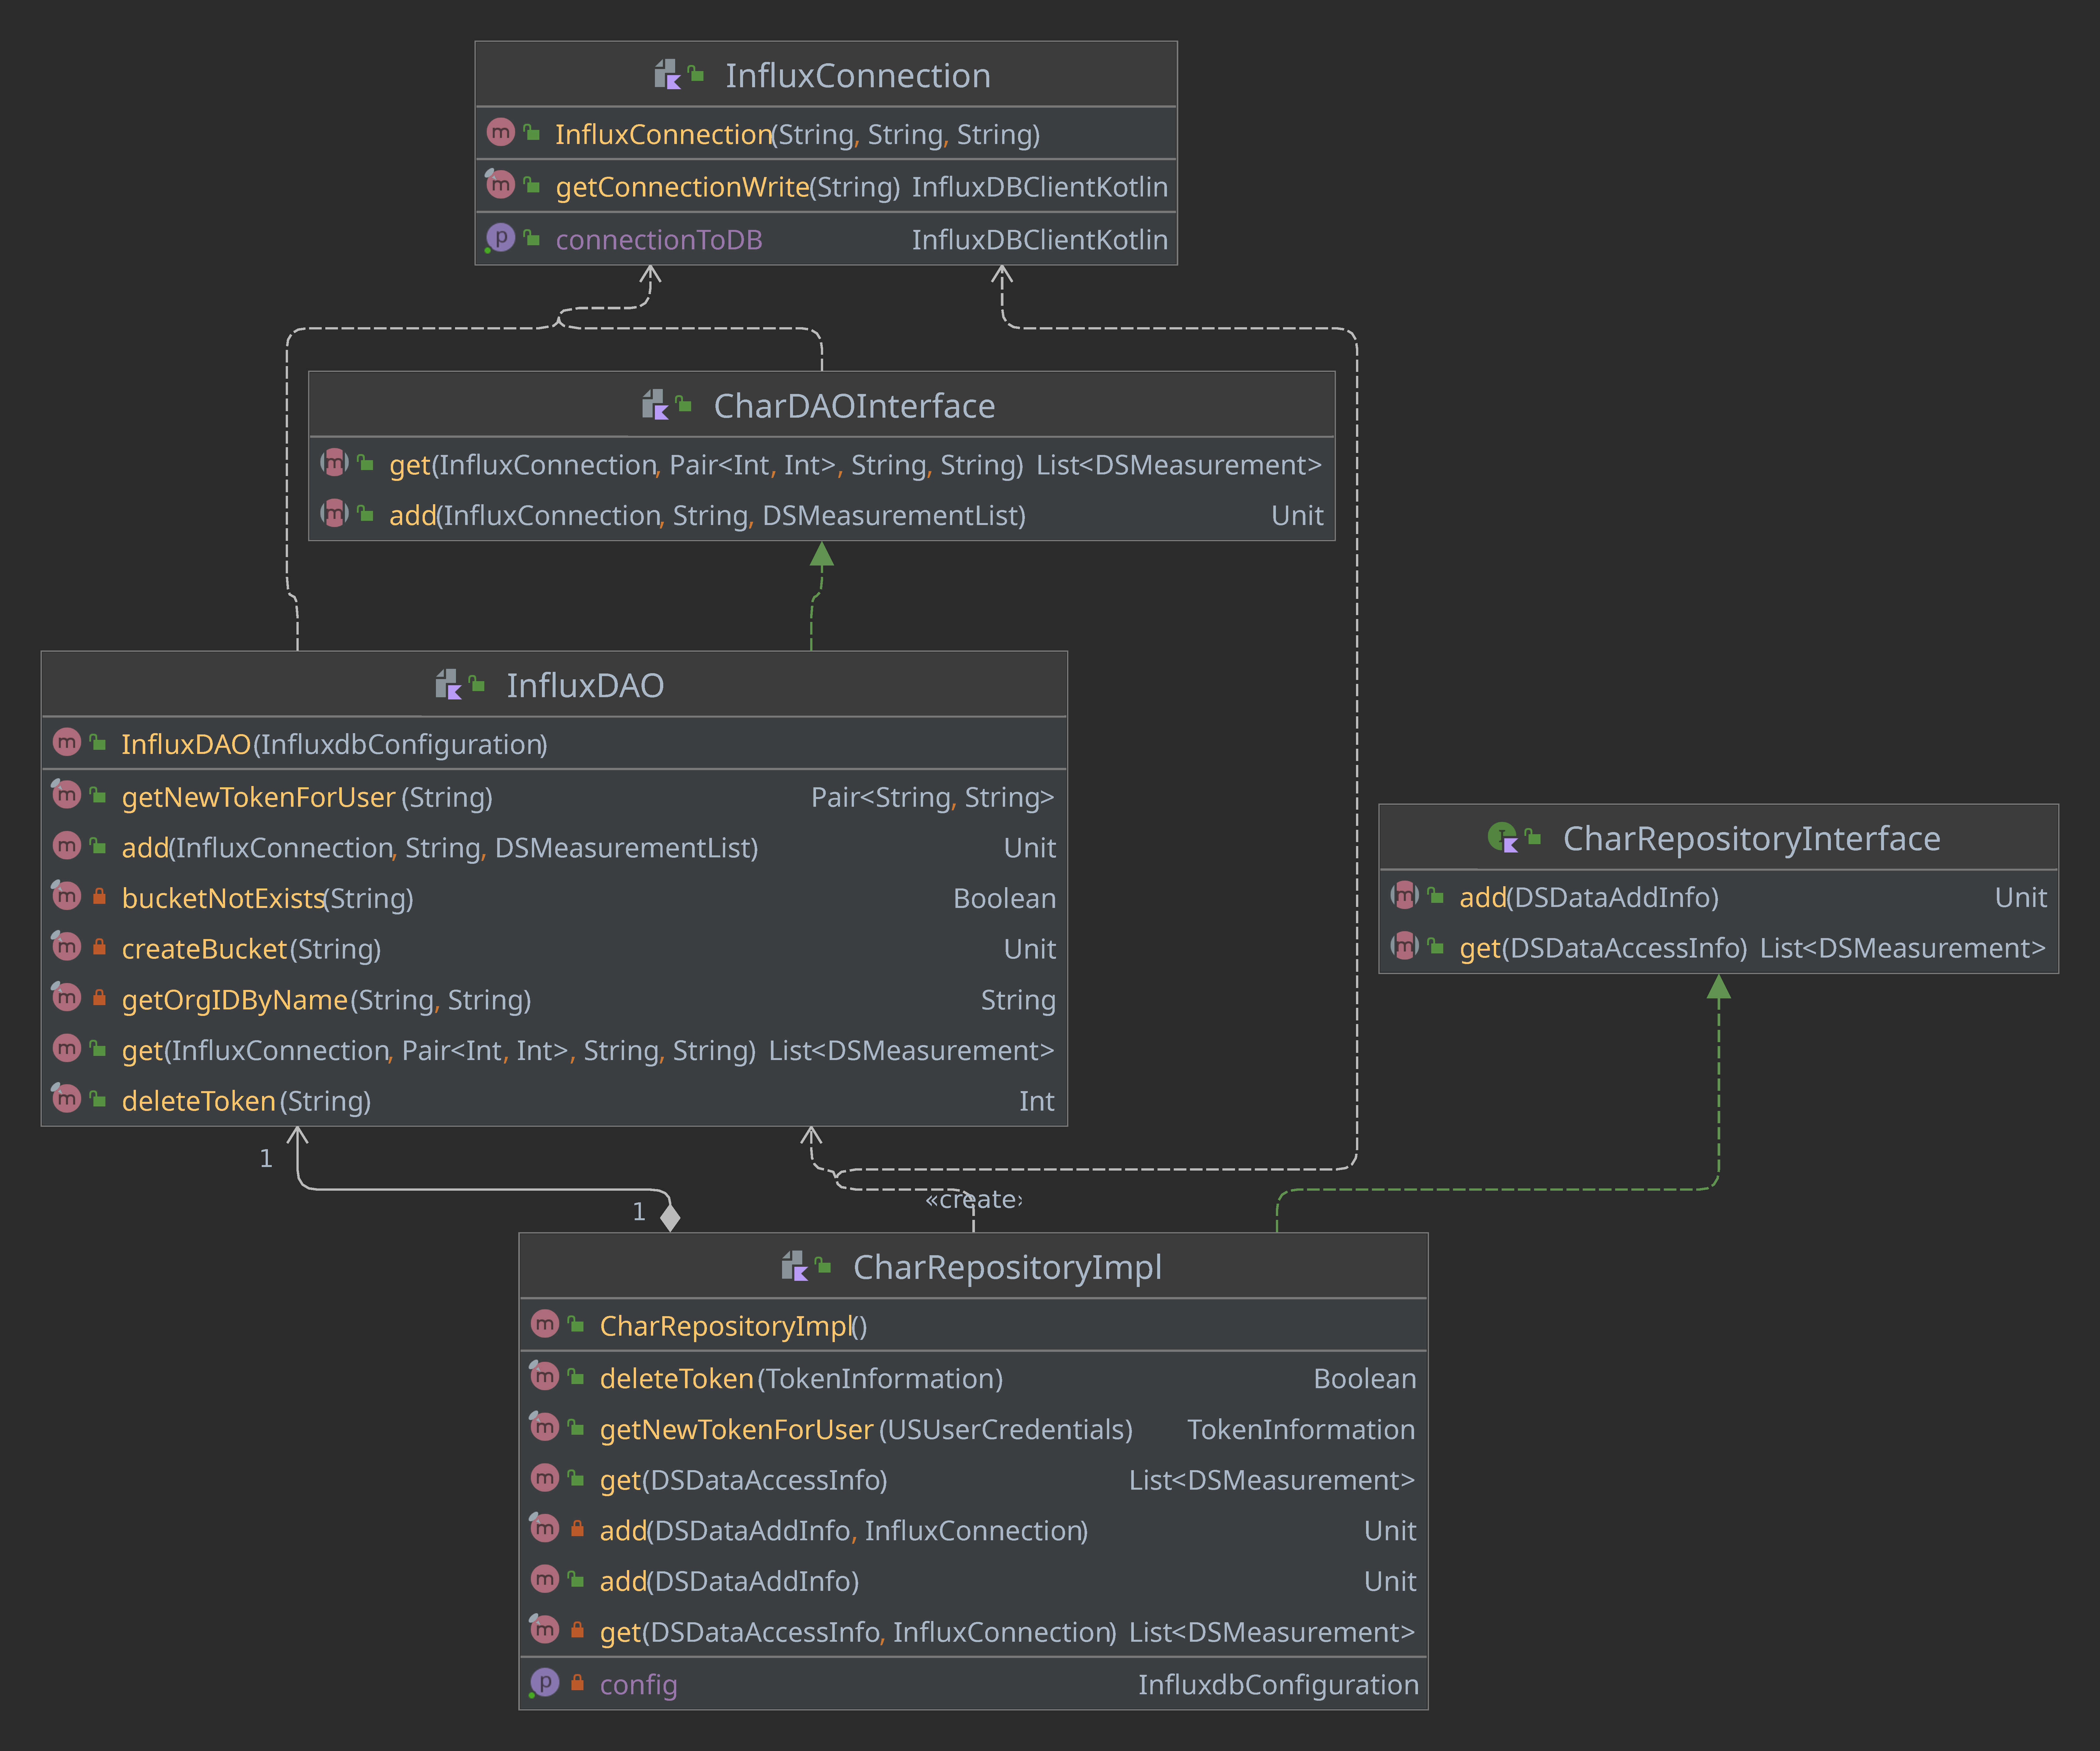
\includegraphics[width=\textwidth]{img/dostup.pdf}
	\caption{Диаграмма классов слоя доступа к данным приложения.}
	\label{fig:dostup}
\end{figure}

\begin{figure}[H]
	\centering
	\includegraphics[width=\textwidth]{img/business.pdf}
	\caption{Диаграмма классов бизнес-логики приложения.}
	\label{fig:business}
\end{figure}

\begin{figure}[H]
	\centering
	\includegraphics[width=\textwidth]{img/svyaz.pdf}
	\caption{Диаграмма классов, показывающая связь контроллера и слоя доступа к данным.}
	\label{fig:svyaz}
\end{figure}

\begin{figure}[H]
	\centering
	\includegraphics[width=\textwidth]{img/server.pdf}
	\caption{Диаграмма классов серверной части приложения.}
	\label{fig:server}
\end{figure}

\subsubsection{Пример использования модулей обработки и анализа данных}

В листинге \ref{lst:analyzemainkt} представлен пример определения текущего состояния \newline пользователя.

На рисунках \ref{fig:analyzeExample0} -- \ref{fig:analyzeExample2} предоставлены все возможные результаты программы.

\begin{figure}[H]
	\centering
	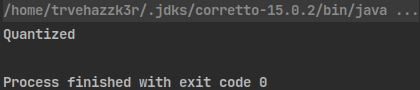
\includegraphics[width=\textwidth]{img/analyzeExample0.png}
	\caption{Результат выполнения, сообщающий о том, что состояние пользователя не установлено.}
	\label{fig:analyzeExample0}
\end{figure}

\begin{figure}[H]
	\centering
	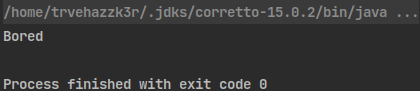
\includegraphics[width=\textwidth]{img/analyzeExample1.png}
	\caption{Результат выполнения, сообщающий о том, что пользователь устал.}
	\label{fig:analyzeExample1}
\end{figure}

\begin{figure}[H]
	\centering
	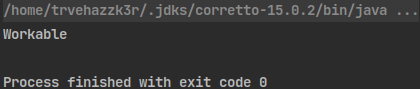
\includegraphics[width=\textwidth]{img/analyzeExample2.png}
	\caption{Результат выполнения, сообщающий о том, что пользователь работоспособен.}
	\label{fig:analyzeExample2}
\end{figure}

\subsubsection{Пример использования серверной части приложения}

В листингах \ref{lst:serverExample} (приложение А, с. \pageref{chp:application-a}) и \ref{lst:clientExample} (приложение А, с. \pageref{chp:application-a}) представлен пример реализации взаимодействия пользователя с сервером.

На рисунках \ref{fig:serverExample} и \ref{fig:clientExample}

\begin{figure}[H]
	\centering
	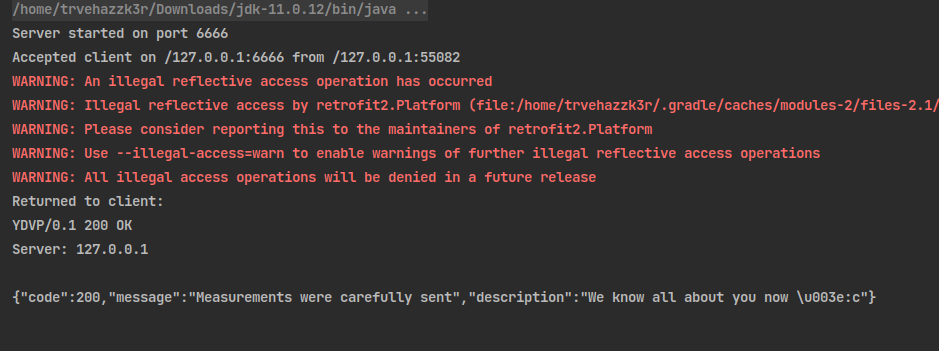
\includegraphics[width=\textwidth]{img/serverOutput.png}
	\caption{Результат выполнения запроса на стороне сервера.}
	\label{fig:serverExample}
\end{figure}

\begin{figure}[H]
	\centering
	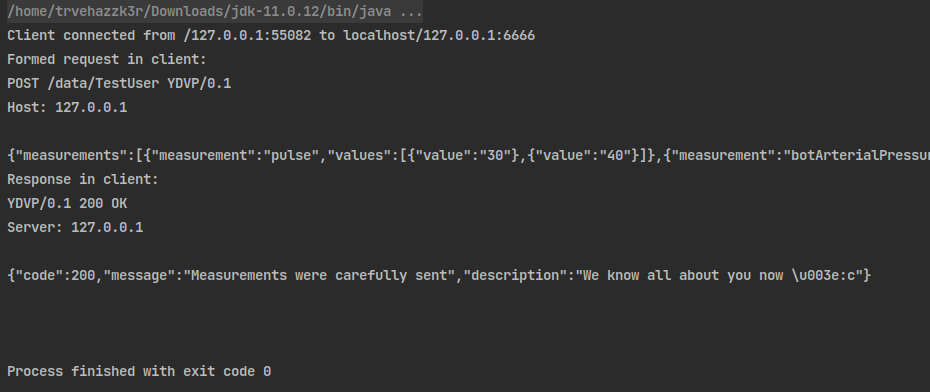
\includegraphics[width=\textwidth]{img/clientOutput.png}
	\caption{Результат выполнения запроса на стороне клиента.}
	\label{fig:clientExample}
\end{figure}

\subsection*{Вывод}
В качестве средства реализации был выбран язык программирования \newline Kotlin, использовалась среда разработки IntelliJ IDEA.

В качестве используемой базы данных была выбрана база данных временных рядов, так как они нацелены на хранение, извлечение и анализ большого количества статистических данных. В качестве СУБД было решено использовать InfluxDB в силу отсутствия аналогов, а также по причине того, что поддержка данной СУБД все еще не прекращена на сегодняшний день.

В качестве алгоритма был выбран метод c-средних в силу того, что число кластеров заранее известно, а также задача рассматривает установку соответствия некоторого объекта набора вещественных значений, показывающих степень отношения объекта к кластерам.

Было определено, что в качестве данных для кластеризации используются действия оператора автоматизированного рабочего места, производимые с использованием клавиатуры и мыши.

Были приведены сведения и особенности модулей логирования действий оператора, анализа данных, серверного приложения.

Также были приведены примеры, которые показали возможные пути использования реализованных компонентов.
